\documentclass[12pt,a4paper]{article}
\usepackage{ctex}
\usepackage{amsmath}
\usepackage{algorithmic} 
\usepackage{amssymb}
\usepackage{graphicx}
\usepackage{booktabs}
\usepackage{geometry}
\usepackage{float}
\usepackage{subcaption}
\usepackage{listings}
\usepackage{hyperref}

\geometry{a4paper,left=2.5cm,right=2.5cm,top=2.5cm,bottom=2.5cm}

\title{月球软着陆控制系统综合仿真实验}
\author{姓名:XXX\\学号:XXX}
\date{\today}

\begin{document}
\maketitle

\begin{abstract}
本实验通过建立月球软着陆动力学模型,设计了基于多项式显式制导的燃耗次优控制方案,
通过MATLAB对主制动段进行仿真,分析了推力偏差(±10\%)和比冲偏差(±10\%),
以及初始速度方向对软着陆过程的影响。实验结果表明,推力增大会缩短制动时间但增加燃料消耗,
比冲降低会导致燃料效率下降,初始速度方向当向x轴偏转只会影响终端经度,
当向y轴偏转则会影响径向速度导致飞行轨迹难以控制,终端位置误差主要来源于横向速度的收敛特性。
该实验代码已开源于\url{https://github.com/LiuZiyue1016/Lunar-soft-landing-control}
\end{abstract}

\textbf{关键词:月球软着陆、动力学模型、多项式显式制导、燃耗次优控制}

\section{引言}
在月球探测带来巨大利益的驱使下,世界各国纷纷出台了自己的探月计划,再一次掀起了新一轮探月高潮。
在月球上着陆分为两种,一种称为硬着陆,顾名思义,就是探测器在接近月球时不利用制动发动机减速而直接撞击月球。
另一种称为软着陆,这种着陆方式要求探测器在距月面一定高度时开启制动系统,把探测器的速度抵消至零,
然后利用小推力发动机把探测器对月速度控制在很小的范围内,从而使其在着陆时的速度具有几米每秒的数量级。

显然,对于科学研究,对探测器实施月球软着陆的科学价值要大于硬着陆。本实验基于绕月停泊轨道方案,
重点研究主制动段的制导控制策略。通过建立轨道坐标系下的非线性动力学模型,采用多项式显式制导方法,
实现燃料次优控制。

\section{理论模型}
\subsection{动力学方程}
在轨道坐标系下,探测器动力学方程描述了探测器在月球引力作用下,受发动机推力影响的运动特性,具体形式如下:

\begin{equation}
\begin{cases}
\dot{r} = u \\
\beta = \frac{v}{r} \\
\dot{\alpha} = \frac{w}{r \sin \beta} \\
\dot{u} = \frac{F \cos \psi}{m} - \frac{\mu}{r^2} + \frac{v^2 + w^2}{r} \\
\dot{v} = \frac{F \sin \psi \cos \phi}{m} - \frac{uv}{r} + \frac{w^2}{r \tan \beta} \\
\dot{m} = -\frac{F}{I_{sp} g_E}
\end{cases}
\end{equation}

其中:
\begin{itemize}
    \item \(r\)、\(\alpha\)、\(\beta\) 分别表示探测器的月心距、月球经度和纬度,定义了探测器在轨道坐标系中的位置。
    \item \(u\)、\(v\)、\(w\) 分别为探测器在径向、切向和垂直方向的速度分量,描述了探测器的运动状态。
    \item \(F\) 表示发动机的推力大小,\(\psi\) 和 \(\phi\) 分别为推力在轨道坐标系中的径向和切向方向角,决定了推力的方向。
    \item \(m\) 为探测器的质量,随燃料消耗而变化。
    \item \(\mu\) 为月球的引力常数,\(I_{sp}\) 为发动机的比冲,\(g_E\) 为地球表面的重力加速度。
\end{itemize}

\subsection{制导律设计}
月球软着陆主制动段的制导律设计旨在高效抵消探测器初始速度,实现燃料最优消耗,
并确保终端状态满足软着陆要求。本设计基于简化动力学模型,采用多项式显式制导方法,具体步骤如下:

\subsubsection{动力学模型简化}
\begin{enumerate}
    \item \textbf{径向动力学方程}:假设月球引力场均匀,引力加速度为常量 \(\mu/R_L^2\),径向动力学方程简化为:
    \begin{equation}
        \ddot{r} = \frac{F u \cos \psi}{m} - \frac{\mu}{R_L^2} 
        \label{eq:radial_dynamics}
    \end{equation}
    其中,\(r\) 为月心距,\(u\) 为径向速度,\(\psi\) 为推力方向角,\(F\) 为发动机推力,\(m\) 为探测器质量。

    \item \textbf{推力加速度展开}:考虑探测器质量变化,推力加速度作一阶泰勒展开:
    \begin{equation}
        \frac{F}{m} \approx \frac{F}{m_0} \left( 1 + \frac{F t}{m_0 C} \right)
        \label{eq:thrust_expansion}
    \end{equation}
    其中 \(C = I_{sp} g_E\),\(m_0\) 为初始质量。
\end{enumerate}

\subsubsection{多项式轨迹建模}
\begin{enumerate}
    \item \textbf{最优控制角分解}:推力方向角 \(\psi\) 分解为目标速度控制角 \(\psi_0\) 与位置修正角 \(p_1, p_2\):
    \begin{equation}
        \psi = \psi_0 + p_1 + p_2 t
        \label{eq:control_angle}
    \end{equation}
    对应 \(\cos \psi\) 近似展开为:
    \begin{equation}
        \cos \psi \approx \cos \psi_0 - p_1 \sin \psi_0 - p_2 t \sin \psi_0
        \label{eq:cos_approx}
    \end{equation}

    \item \textbf{四次多项式轨迹}:径向最优轨迹由四次多项式表示:
    \begin{equation}
        r(t) = k_0 + k_1 t + k_2 t^2 + k_3 t^3 + k_4 t^4
        \label{eq:quartic_traj}
    \end{equation}
    结合假设 \(p_1 \to 0\) 且 \(\psi_0 \approx 90^\circ\),简化为三次多项式:
    \begin{equation}
        r(t) = k_0 + k_1 t + k_2 t^2 + k_3 t^3
        \label{eq:cubic_traj}
    \end{equation}
    对应径向速度 \(u(t) = k_1 + 2k_2 t + 3k_3 t^2\)。

    \item \textbf{系数确定}:通过初始与终端条件 \(r(0)=r_0, u(0)=u_0, r(t_{go})=r_f, u(t_{go})=u_f\),求解系数:
    \begin{equation}
        k_2 = \frac{3(r_f - r_0 - u_0 t_{go}) - (u_f - u_0)t_{go}}{t_{go}^2}
        \label{eq:coeff_k2}
    \end{equation}
    当前径向加速度为:
    \begin{equation}
        a = 2k_2 = \frac{6(r_f - r_0 - u_0 t_{go}) - 2(u_f - u_0)t_{go}}{t_{go}^2}
        \label{eq:radial_accel}
    \end{equation}
\end{enumerate}

\subsubsection{控制角与剩余时间计算}

\begin{figure}[htbp]
\centering
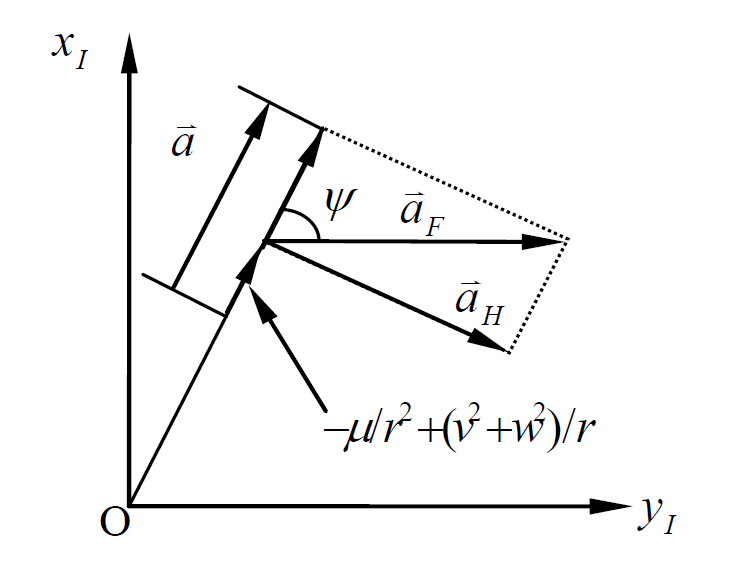
\includegraphics[width=0.8\textwidth]{figures/aF_aH_psi.png}
\caption{加速度矢量几何关系图}
\label{fig:a}
\end{figure}

\begin{enumerate}
    \item \textbf{推力方向角计算}:根据加速度矢量几何关系,推力方向角 \(\psi\) 和 \(\varphi\) 由下式确定:
    \begin{align}
        \psi &= \arccos\left( \frac{a + \mu/r^2 - (v^2 + w^2)/r}{a_F} \right) \\
        \varphi &= \arccos\left( \frac{v_f - v}{\sqrt{(w_f - w)^2 + (v_f - v)^2}} \right)
        \label{eq:control_angles}
    \end{align}
    其中 \(a_F\) 为推力加速度,\(a_H\) 为水平加速度。

    \item \textbf{剩余时间估计}:剩余时间 \(t_{go}\) 近似为水平速度增量与加速度的比值:
    \begin{equation}
        t_{go} = \frac{\sqrt{(w_f - w)^2 + (v_f - v)^2}}{a_H}
        \label{eq:time_to_go}
    \end{equation}
\end{enumerate}

\subsubsection{制导律特点}
\begin{itemize}
    \item \textbf{燃料优化}:基于最优控制理论,通过多项式近似实现燃耗次优。
    \item \textbf{终端约束}:仅约束径向距离与速度,终端位置依赖初始速度精度。
    \item \textbf{鲁棒性}:剩余时间动态更新,适应实时状态变化,但对推力参数偏差敏感。
\end{itemize}

\subsubsection{潜在限制}
\begin{itemize}
    \item \textbf{假设误差}:均匀引力场与一阶近似引入的误差需通过闭环控制补偿。
    \item \textbf{终端突变}:剩余时间趋零时推力角可能突变,需设计末端平滑策略。
    \item \textbf{初始精度要求}:初始速度测量偏差直接影响着陆位置,需高精度导航支持。
\end{itemize}

\section{仿真设计}
\subsection{参数设置}
\begin{itemize}
    \item 初始条件:\(h_0 = 15 \, \text{km}\), \(v_0 = 1692 \, \text{m/s}\), \(m_0 = 600 \, \text{kg}\), \(\beta_0 = 1 \times 10^{-6} \, \text{rad}\), \(\alpha_0 = 5°\), \(u_0 = 0 \, \text{m/s}\), \(w_0 = 0 \, \text{m/s}\)
    \item 终端约束:\(h_f = 2 \, \text{km}\), \(u_f = v_f = w_f = 0 \, \text{m/s}\)
    \item 参数偏差:\(\Delta F = \pm 10\%\), \(\Delta I_{sp} = \pm 10\%\), \(\Delta \theta_{v} = \pm 5°\)
    \item 其他参数:\(F_{\text{nom}} = 1500 \, \text{N}\), \(I_{sp,\text{nom}} = 300 \, \text{s}\), \(g_E = 9.8 \, \text{m/s}^2\), \(\mu = 4.88775 \times 10^{12} \, \text{m}^3/\text{s}^2\), \(R_L = 1738 \, \text{km}\)
\end{itemize}

\subsection{仿真流程}
仿真流程围绕动力学方程展开,重难点在于制导律的迭代计算,核心步骤如下:
\begin{enumerate}
    \item \textbf{初始化}:载入初始状态与终端约束,设定时间步长 \( \Delta t = 0.1 \, \text{s} \) 与收敛容差 \( \epsilon = 10^{-4} \)。
    \item \textbf{制导律迭代}:基于当前状态计算剩余时间 \( t_{\text{go}} \)、推力方向角 \( \psi \),并更新控制指令。
    \item \textbf{动力学传播}:通过四阶龙格-库塔法积分动力学方程,更新探测器状态。
    \item \textbf{终止判断}:若高度 \( h \leq h_f \) 且速度满足终端约束,则终止仿真;否则重复步骤2-3。
\end{enumerate}

\begin{figure}[H]
    \centering
    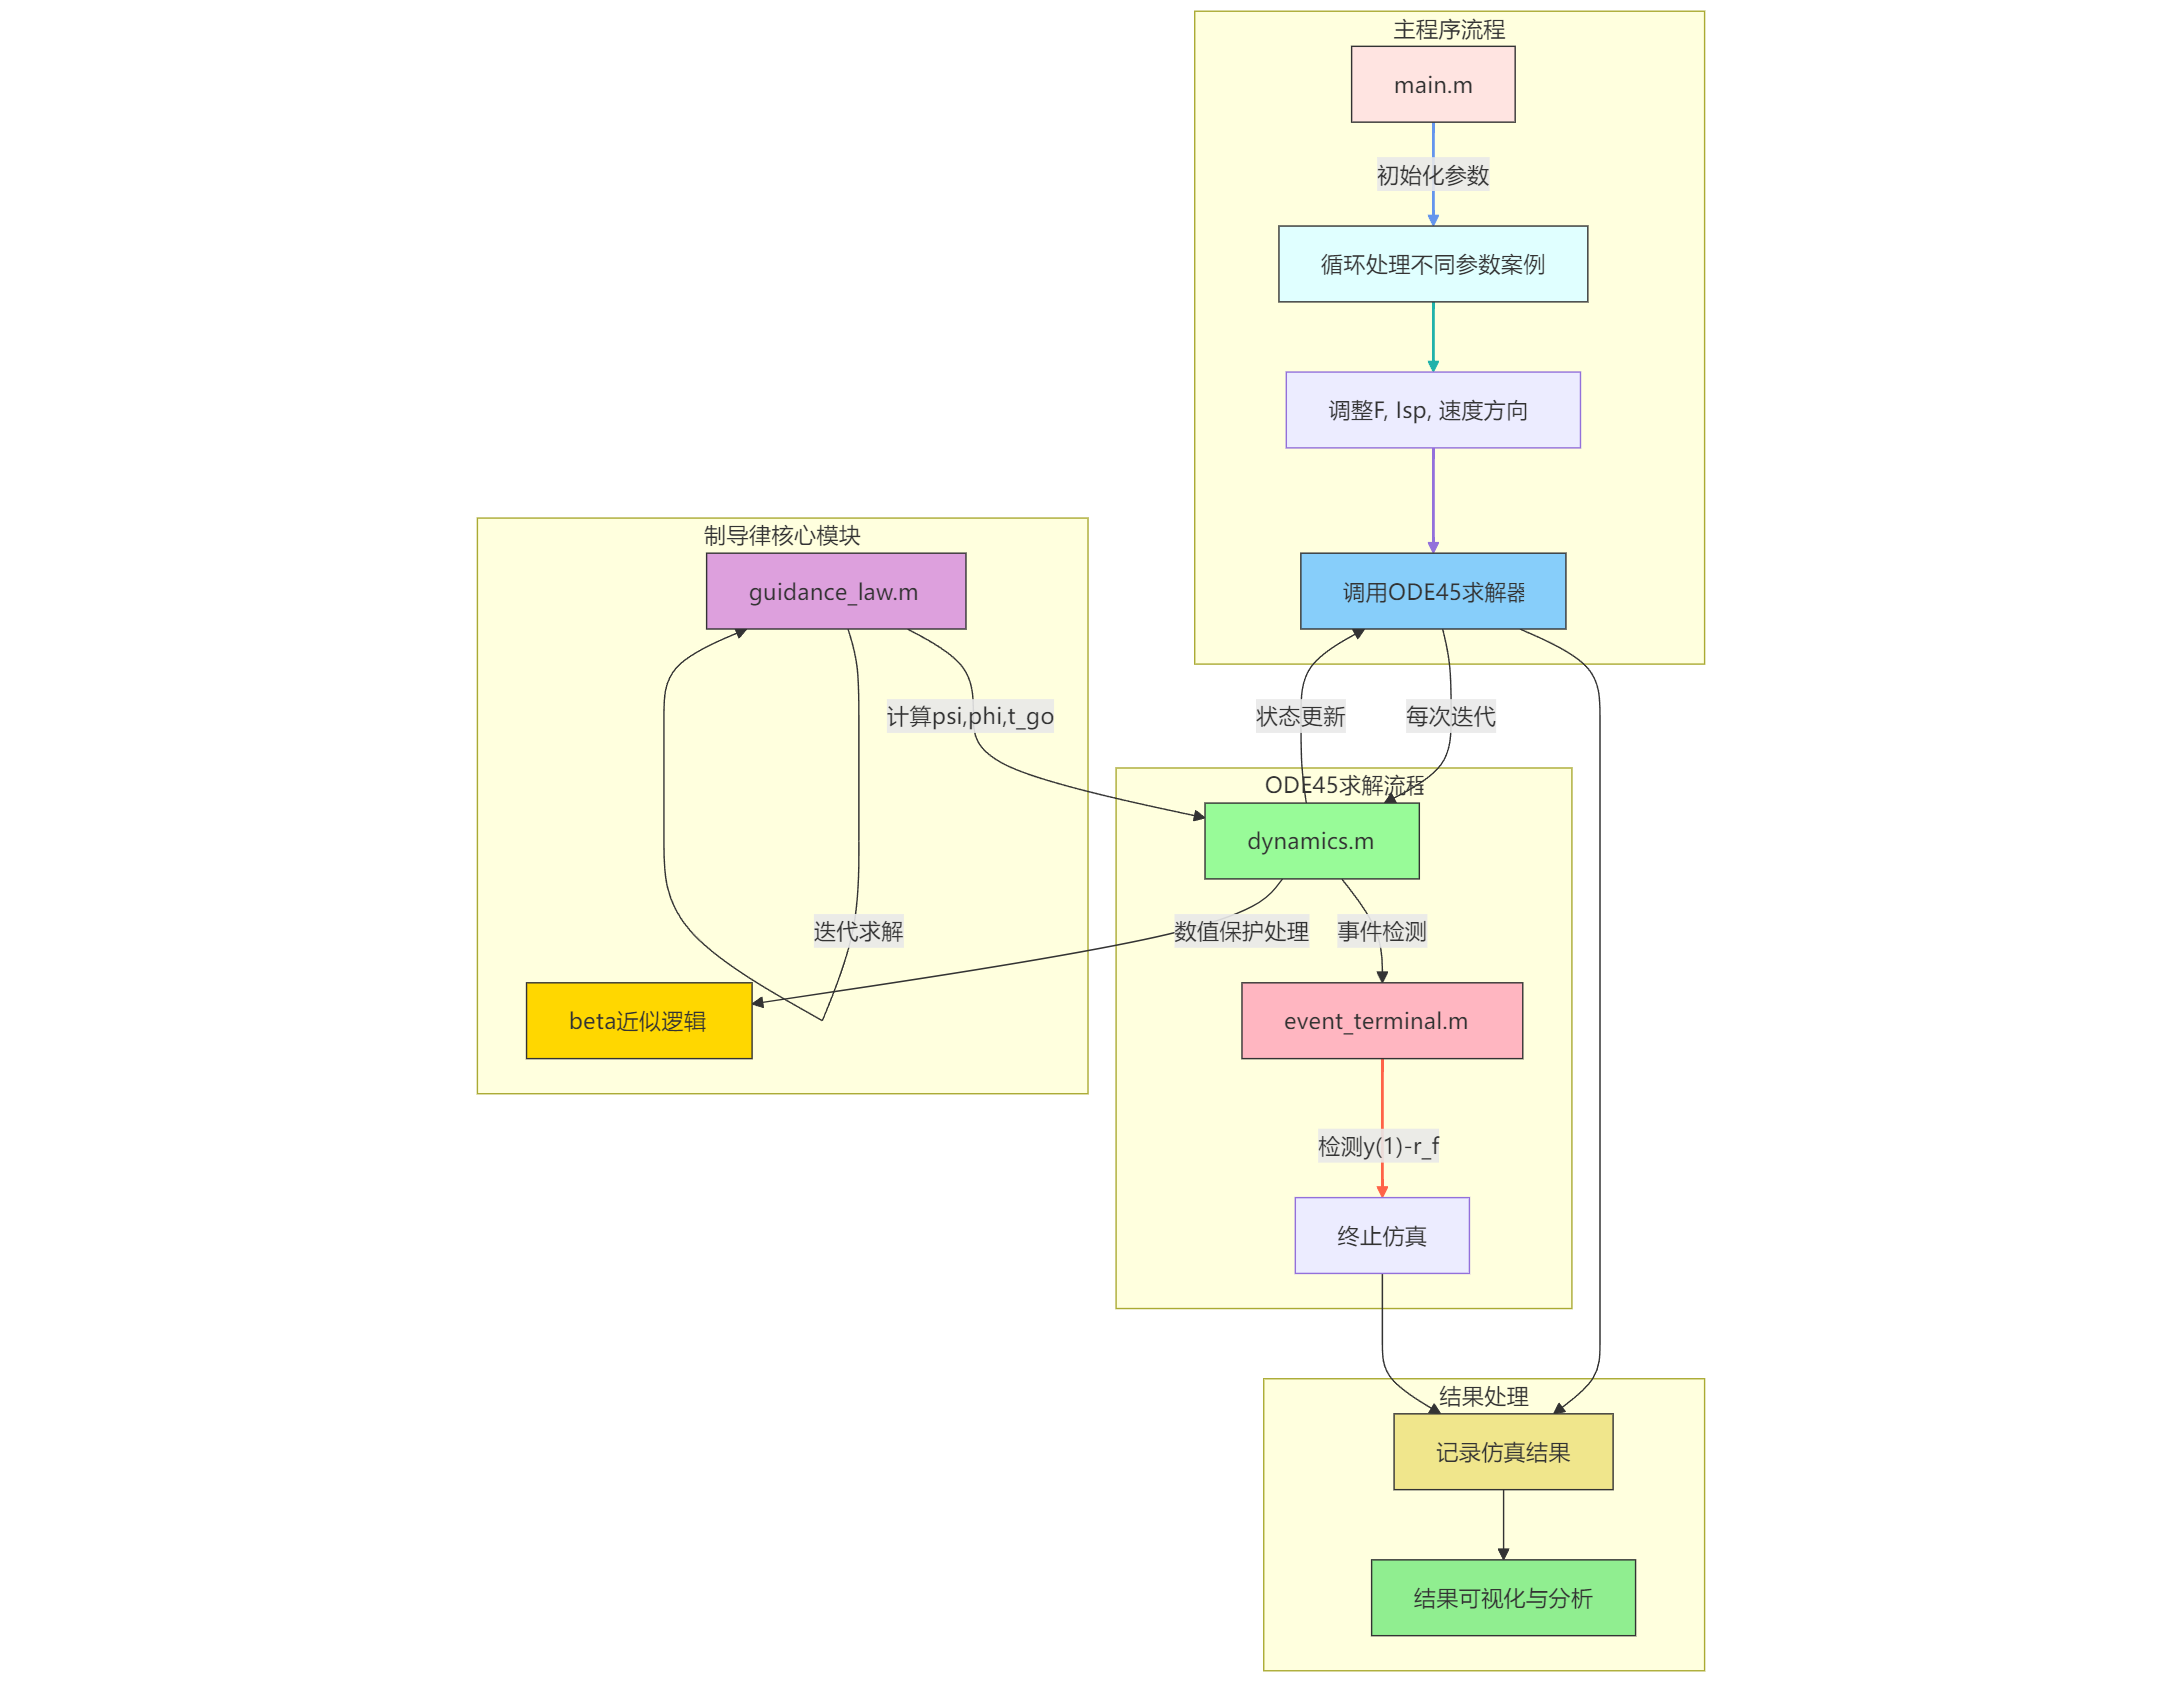
\includegraphics[width=0.85\textwidth]{figures/flowchart.png}  % 替换为实际流程图文件
    \caption{月球软着陆制导控制仿真流程图}
    \label{fig:flow}
\end{figure}

\subsection{制导律迭代流程}
制导律的核心是通过多项式近似求解径向加速度与推力方向角,具体迭代步骤如下:
\begin{verbatim}
while iter < max_iter
    a = (6Δr - 2Δu*t_go) / t_go²      // 计算径向加速度
    ψ = acos((a + μ/r² - (v²+w²)/r)/a_F)
    a_H = a_F * sin(ψ)                // 更新水平加速度
    t_go = sqrt(Δv² + Δw²) / a_H      // 更新剩余时间
    if |t_go_new - t_go| < tolerance
        break
    end
end
\end{verbatim}

\section{结果与分析}
\subsection{探测器轨道}
通过系统仿真,可得到速度、位置、推力方位角等参数随时间的变化曲线。
如图\ref{fig:orbit}所示为着陆器到月心距离随时间变化曲线。着陆器下降到具月球表面2km高度用时538.62s,
下面将分别针对发动机推力、比冲和初始速度方向的偏差,分析其对着陆器飞行过程的影响。
\begin{figure}[H]
\centering
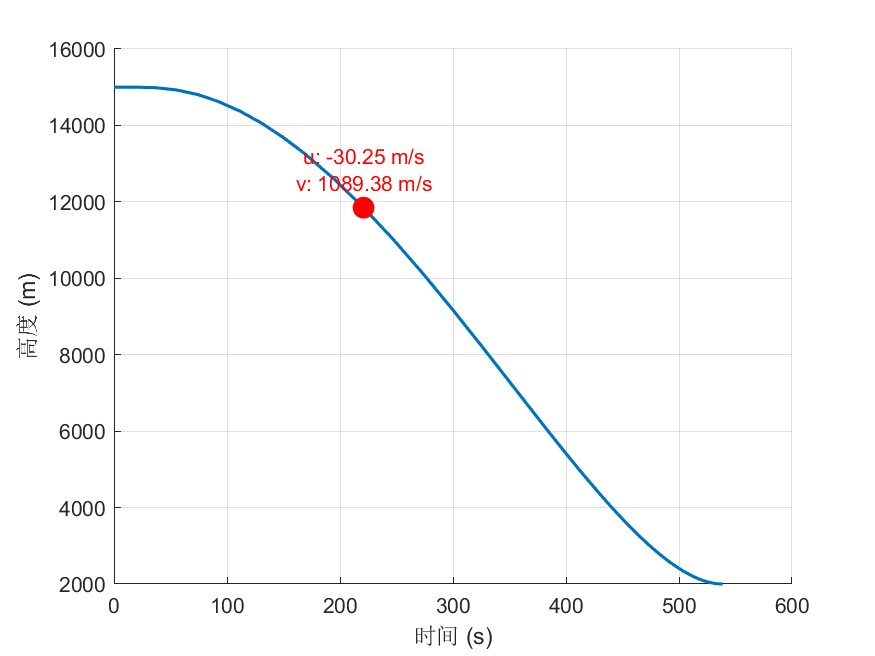
\includegraphics[width=0.8\textwidth]{figures/detector.jpg}
\caption{探测器轨道}
\label{fig:orbit}
\end{figure}

\subsection{发动机推力偏差对软着陆过程的影响}
发动机推力偏差为±10\%,标准推力为1500N,最小推力为1350N,最大推力为1500N。
由于制导控制律不变,着陆器仍然能下降到具月球表面2km的高度,但时间会变化。
由图\ref{fig:altF}可见推力的增大可以缩短探测器下降的时间,推力减小则会增大探测器下降时间。

由于比冲不变,推力变化会引起燃料消耗速度的变化,如图\ref{fig:mF}所示。
然而,由于飞行时间的减小,大推力下总的燃料消耗量会减小。可见采用大推力发动机可以减小燃料的使用量。
但实际情况下还要考虑大推力发动机会不会增加额外的重量,因为推力增大对燃料的节约很有效。
如这个系统中,增大10\%的推力只节约了0.56\%的燃料。

\begin{figure}[H]
\centering
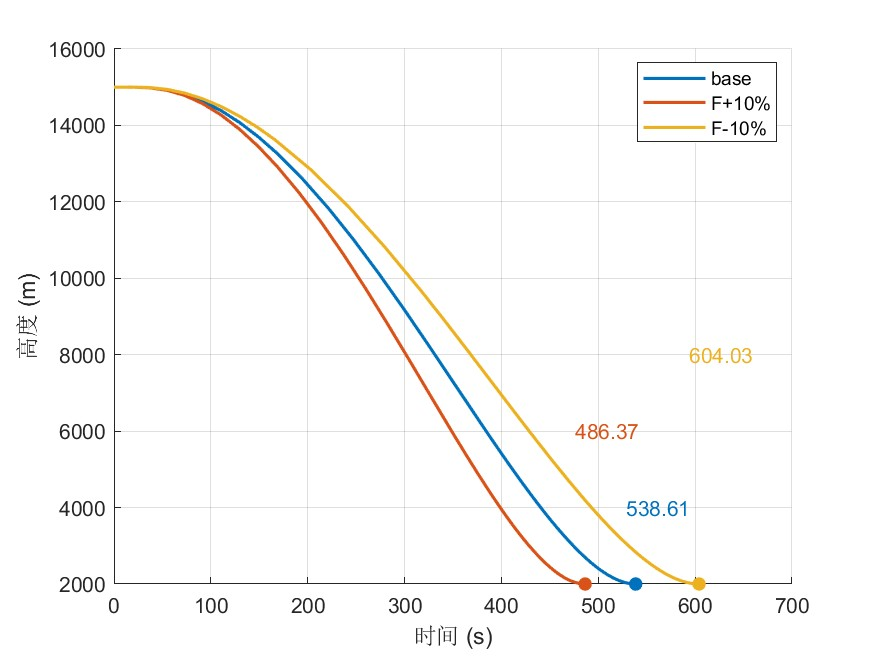
\includegraphics[width=0.8\textwidth]{figures/altitude_F.jpg}
\caption{高度在发动机推力偏差下的变化曲线}
\label{fig:altF}
\end{figure}

\begin{figure}[H]
\centering
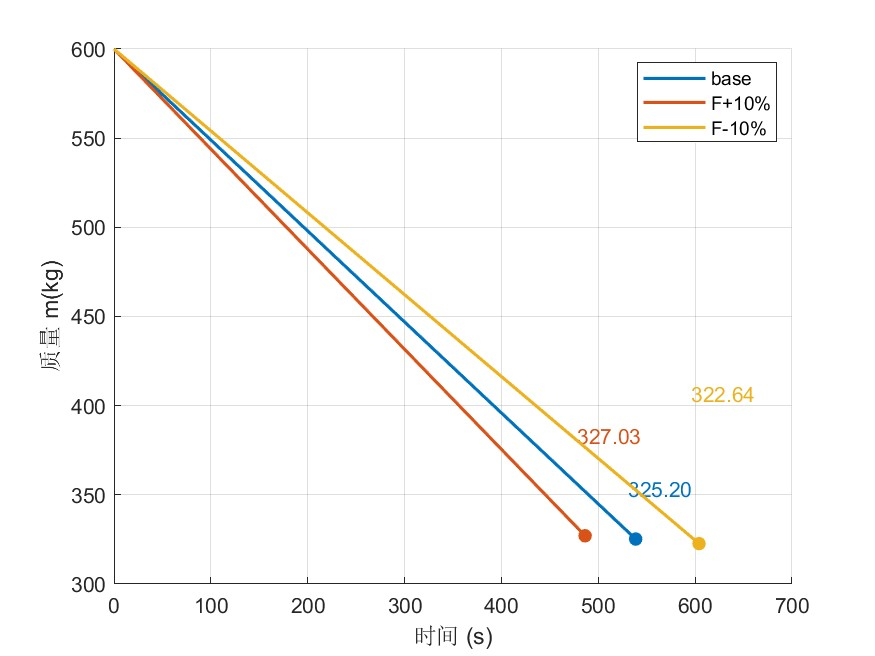
\includegraphics[width=0.8\textwidth]{figures/m_F.jpg}
\caption{燃料质量在发动机推力偏差下的变化曲线}
\label{fig:mF}
\end{figure}

飞行时间的不同最终会导致终点位置的不同,如图\ref{fig:betaF}和\ref{fig:alphaF}所示,但这只会导致纬度的不同,经度不会受到影响,且整个过程经度都不发生改变。

\begin{figure}[H]
\centering
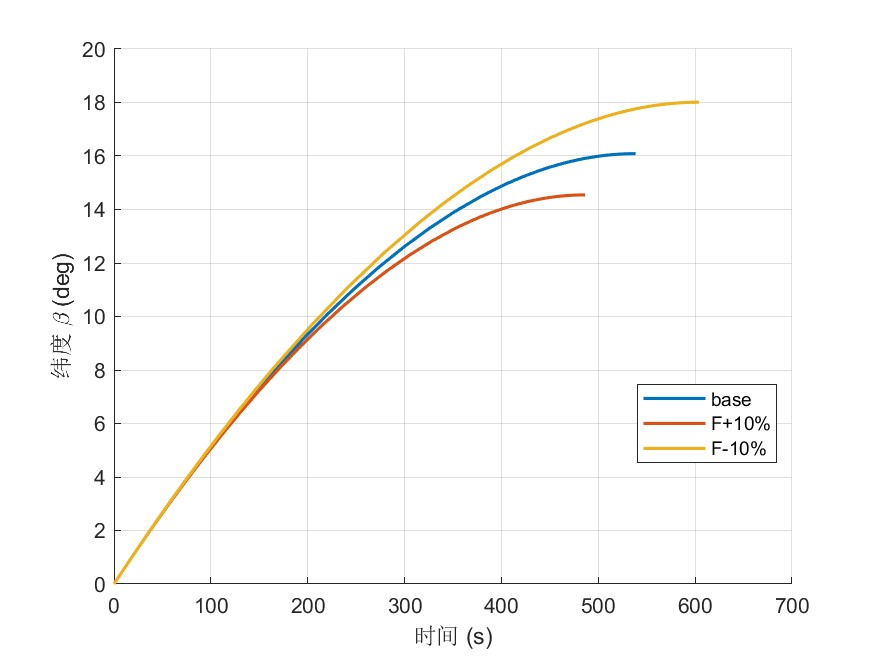
\includegraphics[width=0.8\textwidth]{figures/beta_F.jpg}
\caption{纬度在发动机推力偏差下的变化曲线}
\label{fig:betaF}
\end{figure}

\begin{figure}[H]
\centering
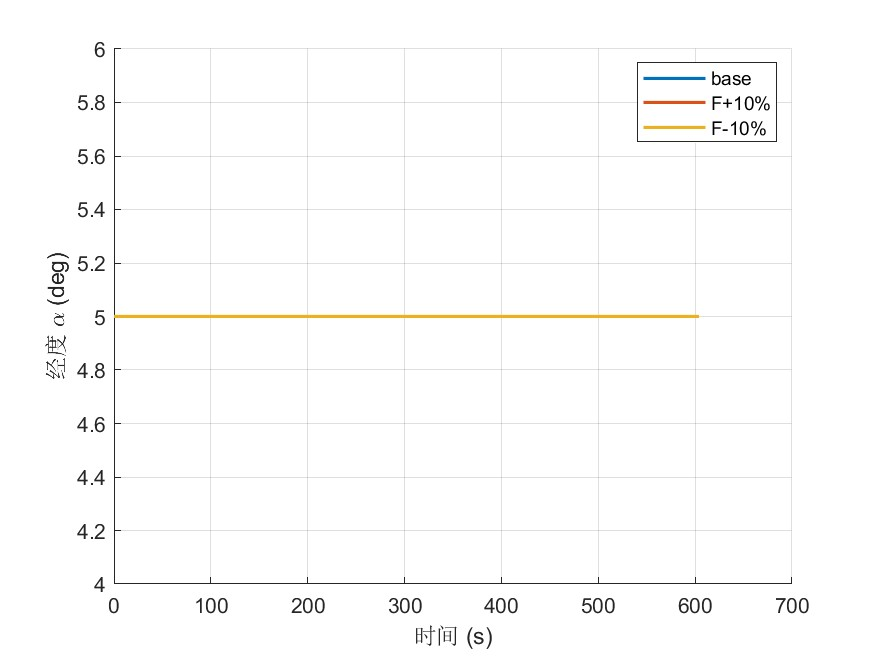
\includegraphics[width=0.8\textwidth]{figures/alpha_F.jpg}
\caption{经度在发动机推力偏差下的变化曲线}
\label{fig:alphaF}
\end{figure}

推力的变化会影响速度变化的快慢,由图\ref{fig:vF}和图\ref{fig:uF}可知,大推力会使速度减小得更快,但缺点是会增大下降时的过载。

从图\ref{fig:uF}可以明显看出下降过程中垂直方向分速度的变化趋势。在减速初期,着陆器会加速下降,末期下降速度会逐渐减小。但无论哪个过程,大推力下加速度都会更大,这也说明了大推力工作时下降过程时间更短的原因。

\begin{figure}[H]
\centering
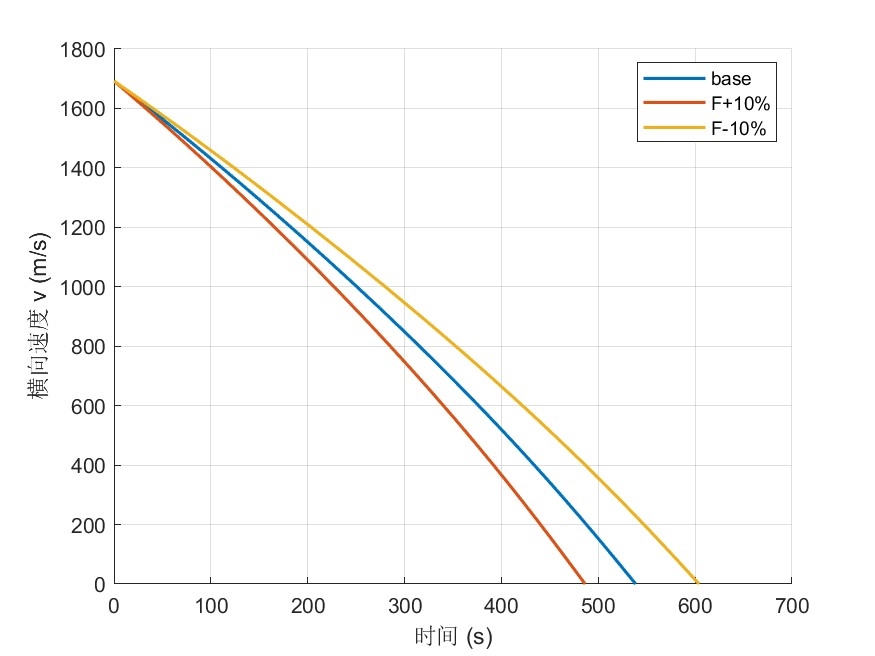
\includegraphics[width=0.8\textwidth]{figures/v_F.jpg}
\caption{横向速度在发动机推力偏差下的变化曲线}
\label{fig:vF}
\end{figure}

\begin{figure}[H]
\centering
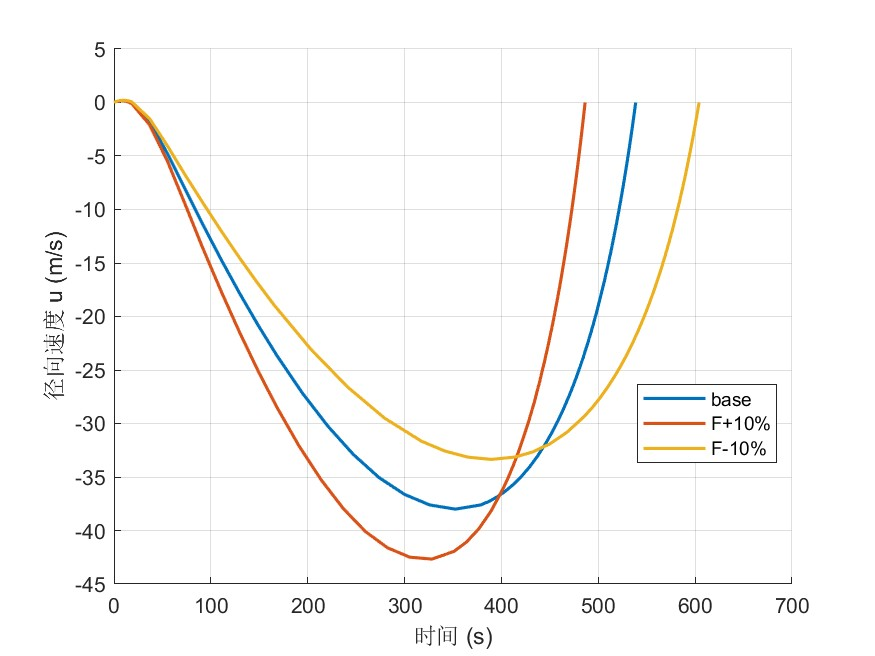
\includegraphics[width=0.8\textwidth]{figures/u_F.jpg}
\caption{径向速度在发动机推力偏差下的变化曲线}
\label{fig:uF}
\end{figure}

\subsection{比冲偏差对软着陆过程的影响}

发动机比冲偏差为±10\%,标准比冲为300,最小比冲为270,最大比冲为330。比冲偏差对着陆过程的影响要小于推力偏差的影响。在相同的推力下,推进剂的比冲越大会延长下降段的时间。这会需要发动机工作更长时间。

但由于当推力一定时,大比冲的推进剂单位时间的消耗量更少,所以综合考虑大比冲推进剂在下降段消耗的推进剂质量更少,如图\ref{fig:altIsp}和\ref{fig:mIsp}所示。

\begin{figure}[H]
\centering
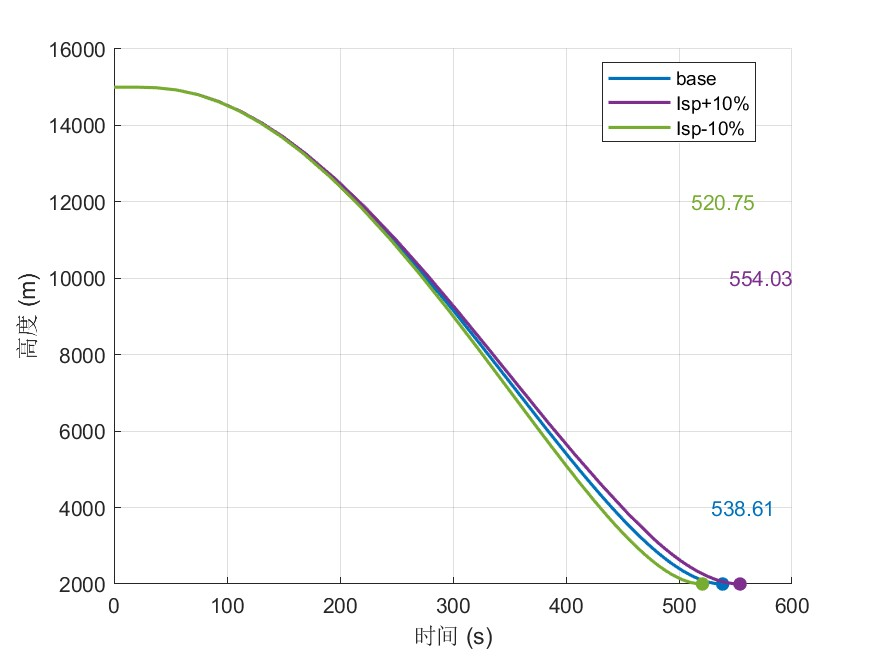
\includegraphics[width=0.8\textwidth]{figures/altitude_Isp.jpg}
\caption{高度在比冲偏差下的变化曲线}
\label{fig:altIsp}
\end{figure}

\begin{figure}[H]
\centering
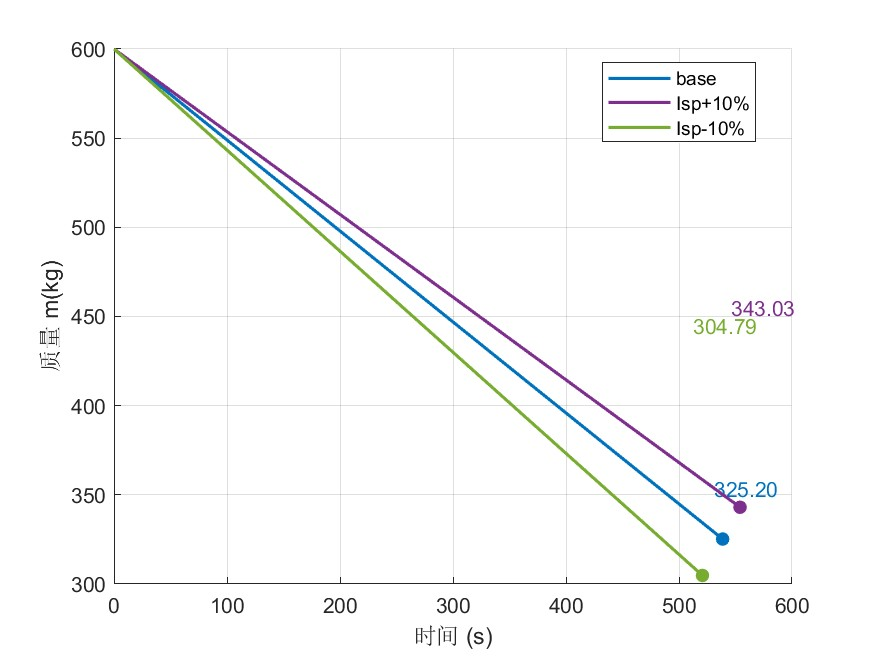
\includegraphics[width=0.8\textwidth]{figures/m_Isp.jpg}
\caption{燃料质量在比冲偏差下的变化曲线}
\label{fig:mIsp}
\end{figure}

如图\ref{fig:betaIsp}和\ref{fig:alphaIsp}所示,与推力偏差对飞行轨迹的影响类似,
飞行时间的不同会导致最终下降的目的地不同。同样这种偏差只会导致纬度的不同,而经度不受影响。
而且飞行时间越短,完成下降段时的纬度越小。

\begin{figure}[H]
\centering
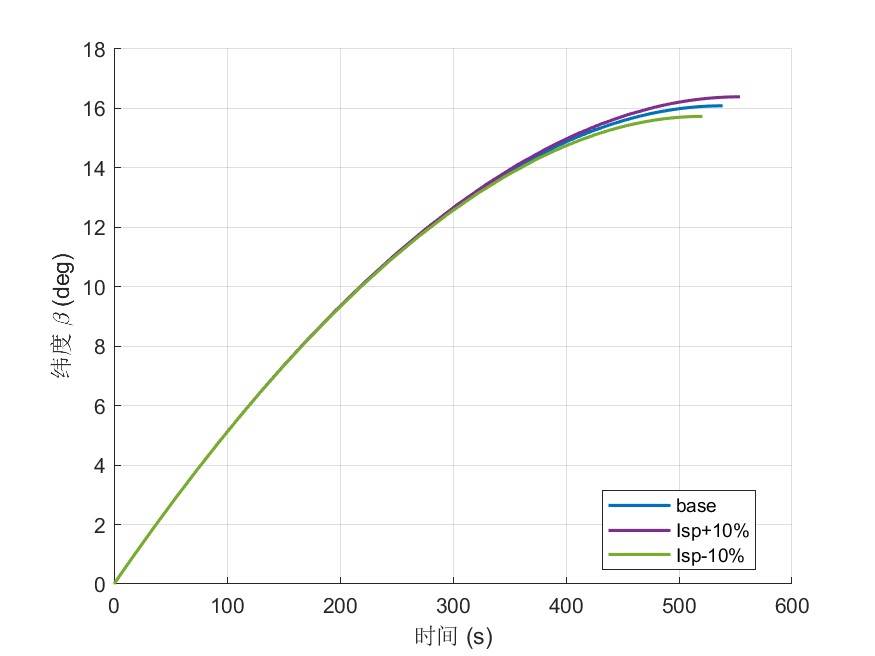
\includegraphics[width=0.8\textwidth]{figures/beta_Isp.jpg}
\caption{纬度在比冲偏差下的变化曲线}
\label{fig:betaIsp}
\end{figure}

\begin{figure}[H]
\centering
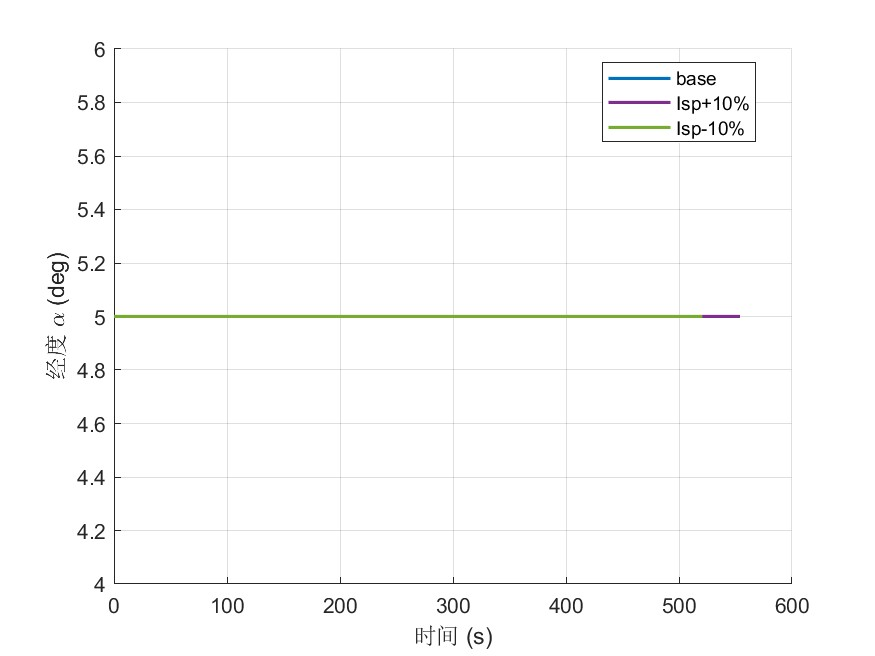
\includegraphics[width=0.8\textwidth]{figures/alpha_Isp.jpg}
\caption{经度在比冲偏差下的变化曲线}
\label{fig:alphaIsp}
\end{figure}

由图\ref{fig:vIsp}和图\ref{fig:uIsp}可见,比冲偏差引起的速度变化与推力偏差类似,
更短的下降时间会产生更多的过载,而当比冲偏大10\%时变化时间最长,所产生负载也就最小。

\begin{figure}[H]
\centering
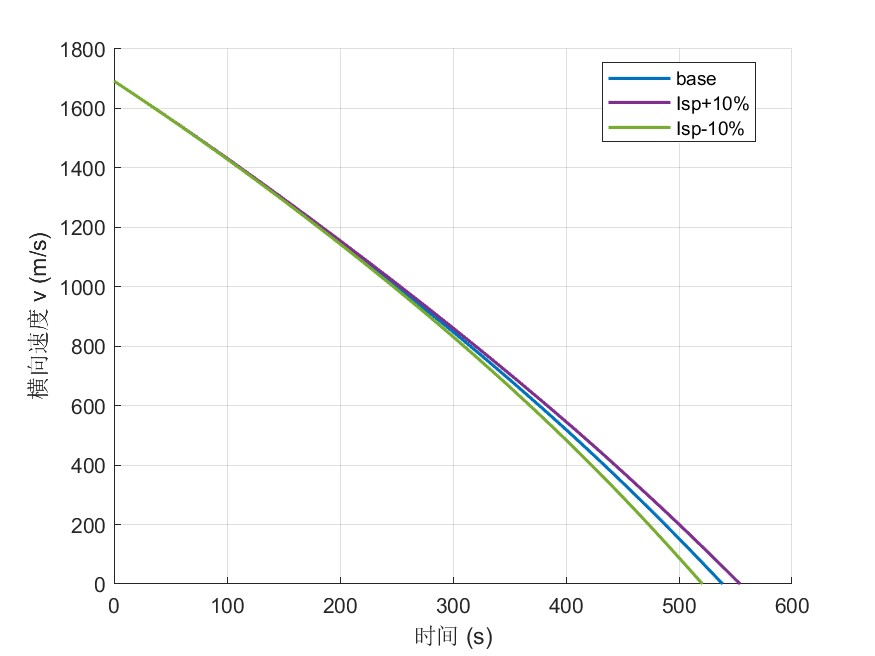
\includegraphics[width=0.8\textwidth]{figures/v_Isp.jpg}
\caption{横向速度在比冲偏差下的变化曲线}
\label{fig:vIsp}
\end{figure}

\begin{figure}[H]
\centering
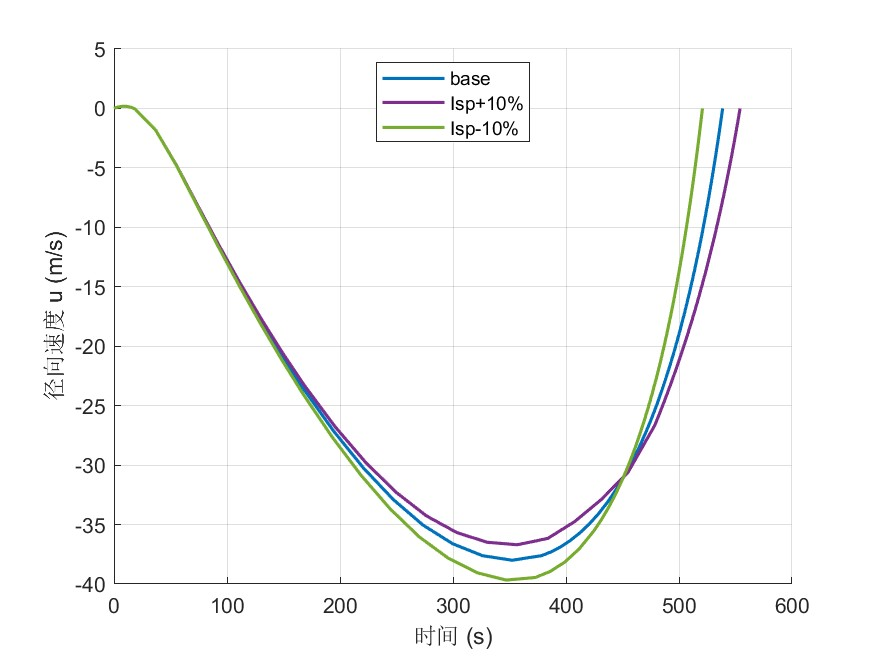
\includegraphics[width=0.8\textwidth]{figures/u_Isp.jpg}
\caption{径向速度在比冲偏差下的变化曲线}
\label{fig:uIsp}
\end{figure}

\subsection{初始速度方向偏差的影响}

为了研究初始速度方向偏差对着陆过程的影响,定义另外两个情况。分别将初始速度向x轴方向偏转5°,
和将初始速度方向朝y轴偏转5°。根据初速度 \( u_0=0 \),\( v_0=1692 \, \text{m/s} \),\( w_0=0 \) 
计算出另外两组初始速度为:
\begin{align*}
u_0 &= 0, & v_0 &= 1686 \, \text{m/s}, & w_0 &= 147.47 \, \text{m/s}; \\
u_0 &= 147.47 \, \text{m/s}, & v_0 &= 1686 \, \text{m/s}, & w_0 &= 0.
\end{align*}
由图\ref{fig:altv}可以看出,着陆器高度的变化曲线不受横向偏航的影响。
着陆器的飞行轨迹与初始的俯仰方向有关。

\begin{figure}[H]
\centering
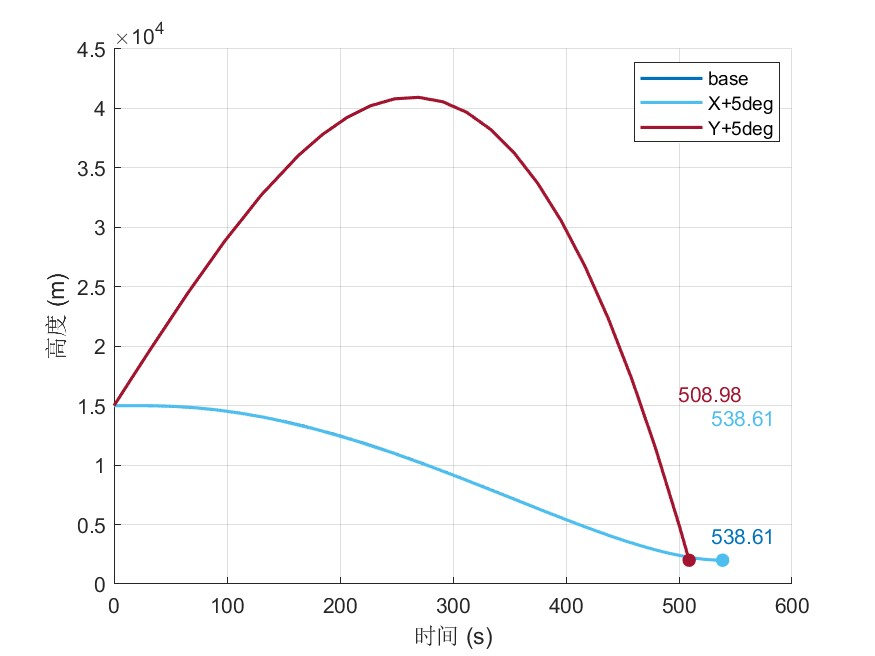
\includegraphics[width=0.8\textwidth]{figures/altitude_VelDir.jpg}
\caption{高度在初始速度方向偏差下的变化曲线}
\label{fig:altv}
\end{figure}

通过观察图\ref{fig:altv},我们发现当径向含有初始速度时,会令探测器先上升再下降,
通过观察图\ref{fig:uv},一方面我们发现径向速度极大,且变化剧烈,不易控制,
另一方面这种飞行方案也会造成燃料的无端浪费。

\begin{figure}[H]
\centering
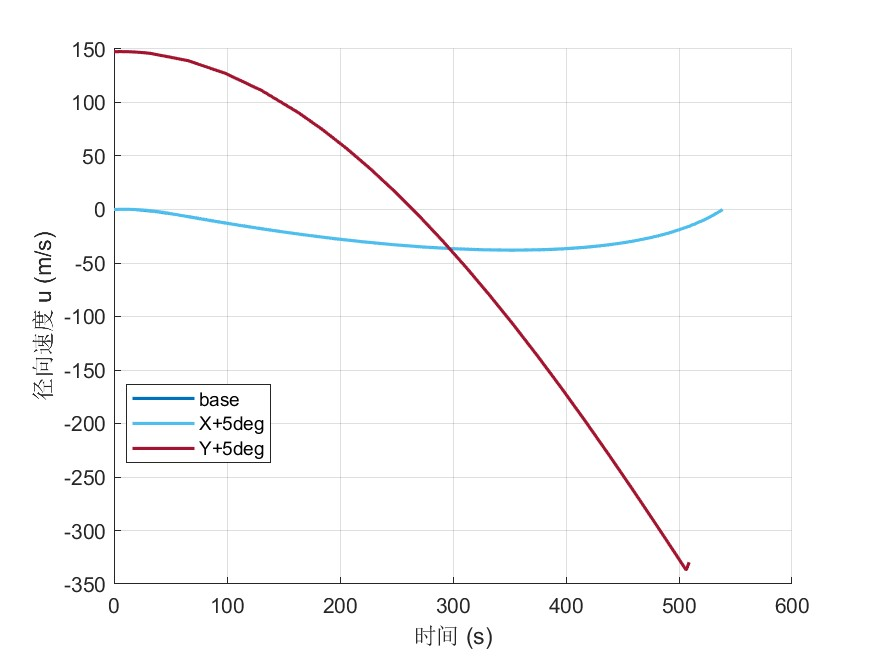
\includegraphics[width=0.8\textwidth]{figures/u_VelDir.jpg}
\caption{径向速度在初始速度方向偏差下的变化曲线}
\label{fig:uv}
\end{figure}

由于发动机的比冲和推力不变,所以速度方向偏差不影响着陆器的质量变化曲线,图\ref{fig:mv}也验证了这一点,
但若初始时刻存在径向速度,尽管造成了燃料的浪费,但由于径向速度极大,剩余燃料反而更多。

\begin{figure}[H]
\centering
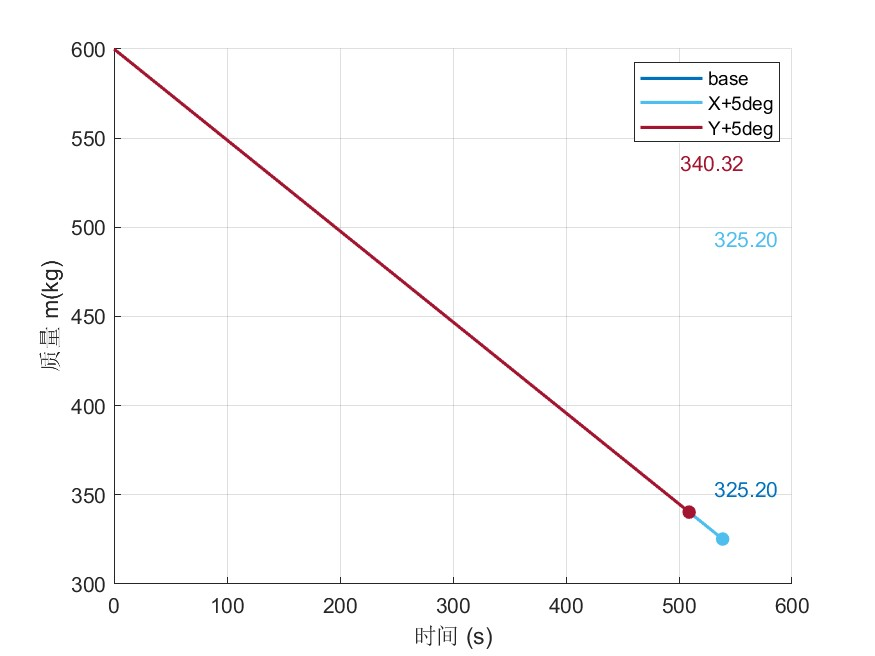
\includegraphics[width=0.8\textwidth]{figures/m_VelDir.jpg}
\caption{燃料质量在初始速度方向偏差下的变化曲线}
\label{fig:mv}
\end{figure}

\subsection{终端位置误差}
\begin{table}[H]
\centering
\caption{终端位置变化与燃料消耗}
\begin{tabular}{cccccccc}
\toprule
Case & F(\%) & Isp(\%) & $X_{angle}$(°) & $Y_{angle}$(°) & $\Delta\alpha$(°) & $\Delta\beta$(°) & 燃料(kg) \\
\midrule
1 & 0   & 0   & 0 & 0 & 0 & 16.0882 & 274.80 \\
2 & +10 & 0   & 0 & 0 & 0 & 14.5458 & 273.97 \\
3 & -10 & 0   & 0 & 0 & 0 & 18.0108 & 277.36 \\
4 & 0   & +10 & 0 & 0 & 0 & 16.3912 & 256.97 \\
5 & 0   & -10 & 0 & 0 & 0 & 15.7326 & 295.21 \\
6 & 0   & 0   & 5 & 0 & 5 & 16.0881 & 274.80 \\
7 & 0   & 0   & 0 & 5 & 0 & 15.0821 & 259.68 \\
\bottomrule
\end{tabular}
\end{table}

\section{结论}
\subsection{推力偏差的影响}
当推力增大10\%时,时间缩短约9.7\%(从538.61 s降至486.37 s),
消耗燃料减少0.56\%(274.80 kg $\to$ 273.97 kg);
而当推力降低10\%,时间则会延长约12.1\%(至604.03 s),
消耗燃料增加0.93\%(274.80 kg $\to$ 277.36 kg)。

通过实验我们发现大推力虽然能缩短时间,但对燃料的节省有限,因此意义不大,有综合评估发动机重量与性能的必要。

\subsection{比冲偏差的影响}
相比发动机推力,比冲对时间的影响很小,对消耗燃料的影响很大,
当比冲减小10\%,消耗燃料增加7.4\%(274.80 kg $\to$ 295.21 kg)。
当比冲增大10\%,消耗燃料减少6.5\%(274.80 kg $\to$ 256.97 kg)。
对于行星际任务来说,推进剂性能的优化对任务经济性具有显著的影响。

\subsection{初始速度方向偏差的敏感性}
当初始速度方向沿x轴偏差5$^\circ$,会导致终端经度偏差约5.0$^\circ$
,需结合高精度导航系统抑制误差。

而当初始速度方向沿y轴偏差5$^\circ$,虽然终端经纬度均不会产生偏差,
但在飞行的过程中,高度会先上升下降到终端位置,其径向加速度极大,不易控制。

\subsection{终端位置误差机制}
\begin{itemize}
    \item \textbf{纬度误差}:主要由横向速度收敛特性决定,偏差范围约$\pm 16^\circ$。
    \item \textbf{经度误差}:受动力学模型简化假设影响较小($\Delta\alpha < 0.1^\circ$)。
    \item \textbf{时间控制}:飞行时间精度达秒级,满足设计要求。
\end{itemize}

\subsection{系统鲁棒性与局限性}
\begin{itemize}
    \item \textbf{敏感参数}:
    \begin{itemize}
        \item 推力偏差需闭环控制补偿引力场假设误差。
        \item 剩余时间趋零时推力角可能突变,需末端平滑策略。
    \end{itemize}
    \item \textbf{适用范围}:燃料次优控制在偏差$\pm 10\%$内仍能保证任务完成,验证工程实用性。
\end{itemize}

\subsection*{优化建议}
\begin{enumerate}
    \item \textbf{控制算法改进}:引入自适应控制动态修正推力方向。
    \item \textbf{多约束优化}:结合终端位置、燃料消耗与时间约束设计综合优化模型。
    \item \textbf{末端策略增强}:添加推力角平滑过渡逻辑以提升稳定性。
\end{enumerate}

\section*{附录}
\subsection*{主代码}
\lstinputlisting[language=Matlab]{code/main.m}

\subsection*{动力学方程}
\lstinputlisting[language=Matlab]{code/dynamics.m}

\subsection*{制导律核心算法}
\lstinputlisting[language=Matlab]{code/guidance_law.m}

\subsection*{其他材料}
本文的完整代码和相关图像文件已托管于
\url{https://github.com/LiuZiyue1016/Lunar-soft-landing-control},
\end{document}